\documentclass{report}
\usepackage[utf8]{inputenc}
\usepackage{hyperref}
\usepackage{graphicx}
\title{User Manual}
\author{Oscar Daniel}
\date{February 2015}
 \graphicspath{ {Images/} }
\begin{document}
 
\maketitle
 
\tableofcontents
 
\chapter{This Product}
 This product is a revision and teaching aid for A Level science subjects, allowing teachers to set their students questions and allow the students access to as many questions as they like. The GUI of this program is designed in a way to allow a user of any technical ability to easily understand and make use of the program.
 


 
\chapter{Installation}
 All computers that will use the program need to have Pyton 3.4 and PyQT 4 installed.\\
 Python 3.4 can be found here : \hyperref[Python Downloads]{https://www.python.org/downloads/}\\
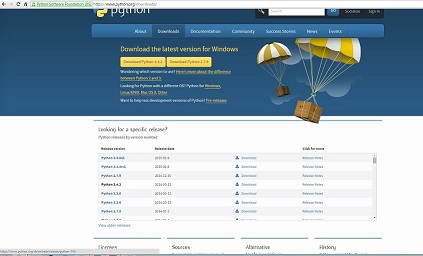
\includegraphics{PythonDownload}\\
 \clearpage
 PyQT 4 can be found here: \hyperref[PyQT]{http://sourceforge.net/projects/pyqt/}\\
 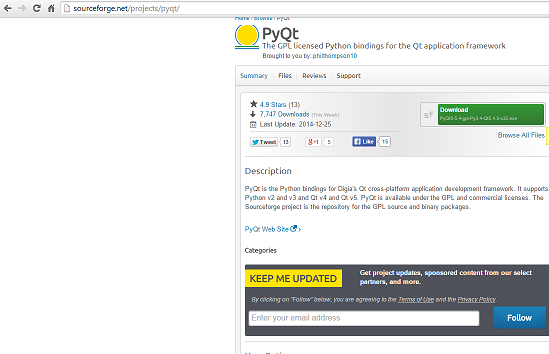
\includegraphics{PyQTDownload}\\
Only Python version 3.4 and Python 3.4 compatible versions of PyQT will work with this program code. Please ensure that you have installed valid distributions before continuing.\\
 
 
\chapter{First Time Setup}
\section{Admin Tools}

\
 
\end{document}